%%%%%%%%%%%%%%%%%%%% book.tex %%%%%%%%%%%%%%%%%%%%%%%%%%%%%
%
% sample root file for the chapters of your "monograph"
%
% Use this file as a template for your own input.
%
%%%%%%%%%%%%%%%% Springer-Verlag %%%%%%%%%%%%%%%%%%%%%%%%%%


% RECOMMENDED %%%%%%%%%%%%%%%%%%%%%%%%%%%%%%%%%%%%%%%%%%%%%%%%%%%
\documentclass[graybox,envcountchap,sectrefs]{svmono}

% choose options for [] as required from the list
% in the Reference Guide

\usepackage{mathptmx}
\usepackage{helvet}
\usepackage{courier}
%
\usepackage{type1cm}         

\usepackage{makeidx}         % allows index generation
\usepackage{graphicx}        % standard LaTeX graphics tool
                             % when including figure files
\graphicspath{{Figures/}}
\usepackage{multicol}        % used for the two-column index
\usepackage[bottom]{footmisc}% places footnotes at page bottom

% see the list of further useful packages
% in the Reference Guide

\makeindex             % used for the subject index
                       % please use the style svind.ist with
                       % your makeindex program
    \addtolength{\oddsidemargin}{-1.25in}
 	\addtolength{\evensidemargin}{-1in}
	\addtolength{\textwidth}{2.5in}

	\addtolength{\topmargin}{0in}
	\addtolength{\textheight}{1.5in}
	
\usepackage{epigraph}
%%%%%%%%%%%%%%%%%%%%%%%%%%%%%%%%%%%%%%%%%%%%%%%%%%%%%%%%%%%%%%%%%%%%%

\begin{document}

\author{Robin. Hartshorne}
\title{Residues and Duality}
\subtitle{based on a seminar on the work of A. Grothendieck}
\maketitle

\frontmatter%%%%%%%%%%%%%%%%%%%%%%%%%%%%%%%%%%%%%%%%%%%%%%%%%%%%%%
\newcommand{\N}{\mathbb{N}}
\newcommand{\R}{\mathbb{R}}
\newcommand{\Q}{\mathbb{Q}}
\newcommand{\Z}{\mathbb{Z}}

\newcommand{\C}{\mathbf{C}}
\newcommand{\PP}{\mathbf{P}}
\newcommand{\HHH}{\mathbf{H}}
\newcommand{\DD}{\mathbf{D}}

\newcommand{\OO}{\mathcal{O}}
\newcommand{\B}{\mathcal{B}}
\newcommand{\cU}{\mathcal{U}}
\newcommand{\F}{\mathcal{F}}
\newcommand{\G}{\mathcal{G}}
\newcommand{\A}{\mathcal{A}}
\newcommand{\CC}{\mathcal{C}}
\newcommand{\DDD}{\mathcal{D}}



\newcommand{\rO}{\mathrm{O}}
\newcommand{\op}{\mathrm{op}}
\newcommand{\rd}{~\mathrm{d}} %roman d
\newcommand{\GL}{\mathrm{GL}}
\newcommand{\SU}{\mathrm{SU}}
\newcommand{\SL}{\mathrm{SL}}
\newcommand{\SO}{\mathrm{SO}}
\newcommand{\U}{\mathrm{U}}
\newcommand{\Sp}{\mathrm{Sp}}
\newcommand{\im}{\mathrm{Im}}
\newcommand{\ord}{\mathrm{ord}}
\newcommand{\End}{\mathrm{End}}
\newcommand{\Aut}{\mathrm{Aut}}
\newcommand{\Hom}{\mathrm{Hom}}
\newcommand{\ad}{\mathrm{ad}}
\newcommand{\tr}{\mathrm{tr}}
\newcommand{\Rad}{\mathrm{Rad}}
\newcommand{\Ext}{\mathrm{Ext}}
\newcommand{\Tor}{\mathrm{Tor}}

\newcommand{\uHom}{\underline{\mathrm{Hom}}}

% \newcommand{\DD}{\overline{\mathbf{D}}}


\newcommand{\res}{\mathsf{res}}



% %%%%%%%%%%%%%%%%%%%%%%% dedic.tex %%%%%%%%%%%%%%%%%%%%%%%%%%%%%%%%%
%
% sample dedication
%
% Use this file as a template for your own input.
%
%%%%%%%%%%%%%%%%%%%%%%%% Springer %%%%%%%%%%%%%%%%%%%%%%%%%%

\begin{dedication}
Use the template \emph{dedic.tex} together with the Springer document class SVMono for monograph-type books or SVMult for contributed volumes to style a quotation or a dedication\index{dedication} at the very beginning of your book in the Springer layout
\end{dedication}





% %%%%%%%%%%%%%%%%%%%%%%foreword.tex%%%%%%%%%%%%%%%%%%%%%%%%%%%%%%%%%
% sample foreword
%
% Use this file as a template for your own input.
%
%%%%%%%%%%%%%%%%%%%%%%%% Springer %%%%%%%%%%%%%%%%%%%%%%%%%%

\foreword

%% Please have the foreword written here
Use the template \textit{foreword.tex} together with the Springer document class SVMono (monograph-type books) or SVMult (edited books) to style your foreword\index{foreword} in the Springer layout. 

The foreword covers introductory remarks preceding the text of a book that are written by a \textit{person other than the author or editor} of the book. If applicable, the foreword precedes the preface which is written by the author or editor of the book.


\vspace{\baselineskip}
\begin{flushright}\noindent
Place, month year\hfill {\it Firstname  Surname}\\
\end{flushright}



%%%%%%%%%%%%%%%%%%%%%%preface.tex%%%%%%%%%%%%%%%%%%%%%%%%%%%%%%%%%%%%%%%%%
% sample preface
%
% Use this file as a template for your own input.
%
%%%%%%%%%%%%%%%%%%%%%%%% Springer %%%%%%%%%%%%%%%%%%%%%%%%%%

\preface

%% Please write your preface here
In the spring of 1963 I suggested to Grothendieck the possibility of my running a seminar at Harvard on his theory of duality for coherent sheaves -- a theory which had been hinted at in his talk to S\'eminaire Bourbaki in 1957 \cite{g1957}, and in his talk to the International Congress of Mathematicians in 1958 \cite{g1958}, but had never been developed systematically. He agreed, saying that he would provide an outline of the material, if I would fill in the details and write up lecture notes of the seminar. During the summer of 1963, he wrote a series of ``pr\'enotes'' which were to be the basis for the seminar.\par
I quote from the preface of the pr\'enotes:
\begin{quote}
    Les presentes notes donnent une esquisse assez d\'{e}taill\'{e}e d'une th\'{e}orie cohomologique de la dualit\'{e} des Modules coh\'{e}rents sur les pr\'{e} sch\'{e}mas. Les id\'{e}es principales de la th\'{e}orie m'etaient connues des 1959, mais le manque de fondements adequats d'Alg\`{e}bre Homologique m'avait emp\^{e}ch\'{e} d'aborder une redaction d'ensemble. Cette lacune de fondements est sur le point d'etre combl\'{e}e par la th\`{e}se de VERDIER, ce qui rend en principe possible un expos\'{e} satisfaisant. Il est d'ailleurs apparu depuis qu il existe des th\'{e}ories cohomologiques de dualit\'{e} formellement tr\`{e}s analogues a celle d\'{e}velopp\'{e}e ici dans toutes sortes d'autres contextes: faisceaux coherents sur les espaces analytiques, faisceaux ab\'{e}liens sur les espaces topologiques (VERDIER), modules galoisiens (VERDIER, TATE), faisceaux de torsion sur les sch\'{e}mas munis de leur topologie \'{e}tale, corps de classe en tous genres... Cela me semble une raison assez s\'{e}rieuse pour se familiariser avec le yoga g\'{e}n\'{e}ral de la dualit\'{e} dans un cas type, comme la th\'{e}orie cohomologique des residus.\par
    La th\'{e}orie consiste pour l'essentiel dans des questions de variance: construction d'un foncteur $f^{!}$ et d'un homomorphisme-trace \[Rf_{\ast}f^{!}\rightarrow id.\] La construction donn\'{e}e ici est compliqu\'{e}e et indirecte et n'est pas valable sous des conditions aussi g\'{e}n\'{e}rales qu'on est en droit de s'y attendre. Il faudra sans doute une id\'{e}e nouvelle pour apporter des simplifications substantielles.
\end{quote}

The seminar took place in the fall and winter of 1963-64, with the assistance of David Mumford, John Tate, Stephen Lichtenbaum, John Fogarty, and others, and gave rise to a series of six expos\'es which were circulated to a limited audience under the title ``S\'eminaire Hartshorne''. The present notes are a revised, expanded, and completed version of the prevoius notes.\par
I would like to take this opportunity to thank all those people who have helped in the course of this work, and in particular A. Grothendieck, who gave continual support and encouragement throughout the whole project.




\vspace{\baselineskip}
\begin{flushright}\noindent
\hfill {\it R. H.}\\
Cambridge, May 1966
\end{flushright}




% %%%%%%%%%%%%%%%%%%%%%%acknow.tex%%%%%%%%%%%%%%%%%%%%%%%%%%%%%%%%%%%%%%%%%
% sample acknowledgement chapter
%
% Use this file as a template for your own input.
%
%%%%%%%%%%%%%%%%%%%%%%%% Springer %%%%%%%%%%%%%%%%%%%%%%%%%%

\extrachap{Acknowledgements}

Use the template \emph{acknow.tex} together with the Springer document class SVMono (monograph-type books) or SVMult (edited books) if you prefer to set your acknowledgement section as a separate chapter instead of including it as last part of your preface.




\tableofcontents

% %%%%%%%%%%%%%%%%%%%%%%acronym.tex%%%%%%%%%%%%%%%%%%%%%%%%%%%%%%%%%%%%%%%%%
% sample list of acronyms
%
% Use this file as a template for your own input.
%
%%%%%%%%%%%%%%%%%%%%%%%% Springer %%%%%%%%%%%%%%%%%%%%%%%%%%

\extrachap{Acronyms}

Use the template \emph{acronym.tex} together with the Springer document class SVMono (monograph-type books) or SVMult (edited books) to style your list(s) of abbreviations or symbols in the Springer layout.

Lists of abbreviations\index{acronyms, list of}, symbols\index{symbols, list of} and the like are easily formatted with the help of the Springer-enhanced \verb|description| environment.

\begin{description}[CABR]
\item[ABC]{Spelled-out abbreviation and definition}
\item[BABI]{Spelled-out abbreviation and definition}
\item[CABR]{Spelled-out abbreviation and definition}
\end{description}


\mainmatter%%%%%%%%%%%%%%%%%%%%%%%%%%%%%%%%%%%%%%%%%%%%%%%%%%%%%%%
% %%%%%%%%%%%%%%%%%%%%%part.tex%%%%%%%%%%%%%%%%%%%%%%%%%%%%%%%%%%
% 
% sample part title
%
% Use this file as a template for your own input.
%
%%%%%%%%%%%%%%%%%%%%%%%% Springer %%%%%%%%%%%%%%%%%%%%%%%%%%

\begin{partbacktext}
\part{Part Title}
\noindent Use the template \emph{part.tex} together with the Springer document class SVMono (monograph-type books) or SVMult (edited books) to style your part title page and, if desired, a short introductory text (maximum one page) on its verso page in the Springer layout.

\end{partbacktext}
\Extrachap{Introduction}
% \epigraph{I recall seeing a package to make quotes}{Snowball}
The main purpose of these is to prove a duality theorem for the cohomology of quasi-coherent sheaves, with respect to a proper morphism of locally noetherian preschemes. Various such theorems are already known. Typical is the duality theorem for a non-singular complete curve $X$ over an algebraically closed field $k$, which say that
\[h^0(D)=h^1(K-D),\]
where $D$ is a divisor, $K$ is the canonical divisor, and 
\[h^{i}(D)=\dim_k H^i(X,L(D))\]
for any $i$, and any divisor $D$. (See e.g. \cite{s1959} Ch. II for a proof.) \par

Various attempts were made to generalize this theorem to varieties of higher dimension, and as Zariski points out in his report \cite{report1956}, his generalization of a lemma of Enriques-Severi \cite{z1952} is equivalent to the statement that for a normal projective variety $X$ of dimension $n$ over $k$,
\[h^0(D)=h^n(K-D)\]
for any divisor $D$. This is also equivalent to a theorem of Serre (See \cite{fac} 76 Thm. 4) on the vanishing of the cohomology group $H^1(X,L(-m))$ for $m$ large and $L$ locally free. Using a related theorem (See \cite{fac} 75 Thm. 3), Zariski shows how one can deduce on a non-singular projective variety the formula
\[h^i(D)=h^{n-i}(K-D)\]
for $0\leq i\leq n$. In terms of sheaves, this result corresponds to the fact that the $k$-vector spaces
\[H^i(X,\F)\quad \textrm{ and } \quad H^{n-i}(X,\F^{\vee}\otimes \omega)\]
are dual to each other, where $\F$ is locally free sheaf, $F^{\vee}$ is the dual sheaf $\cHom(\F,\OO_X)$, and $\omega=\Omega^n_{X/k}$ is the sheaf of $n$-differentials on $X$. Serre gives a proof of this same theorem by analytic methods for a compact complex analytic manifold $X$.\par

Grothendieck gave some generalizations of these theorems for non-singular projective varieties, and then in \cite{} announced the general theorem for schemes proper over a field, with arbitrary singularities, which is the subject of the present lecture notes.\par 

To motivate the statement of our main theorem, let us consider the case of projective space $X=\PP^n_k$ over an algebraically closed field $k$. Then there is a canonical isomorphism
\[H^n(X,\omega)\cong k\]
where $\omega^n_{X/k}$ is the sheaf of $n$-differentials. Combining this with the Yoneda pairing
\[H^i(X,\F)\times \Ext_X^{n-i}(\F,\omega)\rightarrow H^n(X,\omega)\]
we obtain a pairing
\[H^i(X,\F)\times \Ext^{n-i}_X(\F,\omega)\rightarrow k\]
which one shows easily to be a perfect pairing \cite{}. This genarlizes the statements above, becasue for a locally free sheaf $\F$,
\[\Ext^{n-i}(\F,\omega)=\Ext^{n-i}(\OO_X,\F^{\vee}\otimes \omega)=H^{n-i}(X,\F^{\vee}\otimes \omega).\]
Another way of looking at our duality pairing is as an isomorphism
\begin{equation}\label{iso1}\Ext^{n-i}_X (\F,\omega)\rightarrow \Hom_k(H^i(X,\F),k).
\end{equation}
Since everything is linear over $k$, we may introduce a $k$-vector space $G$, and have an isomorphism
\begin{equation}\label{iso}\Ext^{n-i}_X (\F,G\otimes_k\omega)\rightarrow \Hom_k(H^i(X,\F),G).
\end{equation}
Before proceeding further, we must introduce the derived category. It will be discussed in detail in Chapter I, but for the moment it will be sufficient to know the following:

For each abelian category $\A$, there is a category $D(\A)$, called the {\it derived category} of $A$, whose objects are complexes of objects of $A$. If $F:\A\rightarrow \B$ is an additive functor from one abelian category to another, then under reasonable conditions there is a {\it right derived functor} \[RF:D(\A)\rightarrow D(\B)\] 
with the property that for any $X\in Ob(\A)$, if $X$ denotes also the complex which is $X$ in degree zero, and zero elsewhere, then $H^i(RF(X))=R^iF(X)$, where $R^iF$ is the ordinary $i$-th right derived functor of $F$. Finally, if $F:\A\to \B$ and $G:\B\to \CC$ are two functors then 
\[R(G\circ F)=R(G)\circ R(F).\]
This replaces the old-fashioned spectral sequence of a composite functor.

Now we can jazz up our duality for projective space as follows. We replace $k$ by a prescheme $Y$, so that $X=\PP^n_Y$. We consider the derived categories $D(X)$ and $D(Y)$ of the categories of $\OO_X$-modules and $\OO_Y$-modules, respectively. Then cohomology $H^i$ becomes $Rf_*$, the derived functor of the direct image functor $f_*$, where $f:X\to Y$ is the projection. The functor $\Ext$ becomes the derived functor $R\Hom$ of $\Hom$. We define
\[f^{!}(G)=f^*(G)\otimes \omega,\]
for $G\in D(Y)$, and we replace $F$ by a complex of sheaves $F\in D(X)$. Then the isomorphism $H^n(X,\omega)\cong k$ gives us an isomorphism
\[Rf_*f^!G \xrightarrow{\sim} G \]
which we call the {\it trace map}. The Yoneda pairing reappears as a natural map 
\begin{equation}\label{map1}
R\Hom_X(F,f^!G) \longrightarrow R\Hom_Y(Rf_*F,Rf_*f^!G),
\end{equation}
which, composed with the trace map gives us the {\it duality morphism}
\[R\Hom_X(F,f^!G) \longrightarrow R\Hom_Y(Rf_*F,G)\]
which generalize \ref{iso}. This is easily proved to be an isomorphism (III 5.1 below) under the suitable hypotheses on $Y,~F,~G$. In fact, the proof is nothing but ``general nonsense'' once one has the isomorphism \ref{iso1}.

Having examined the case of projective space, we can state the following ideal theorem, which is the primum mobile of these notes, although it may never appear explicitly in this form.

(adjust the symbol, cohomology of sheaf, Hom sheaf and Hom set, eliminate the underline )

\begin{theorem}[Ideal Theorem]
\begin{enumerate}[(a)]
\item For every morphism $f:X\to Y$ of finite type of preschemes, there is a functor
\[f^!:~D(Y)\to D(X)\]
such that
 \begin{enumerate}[1)]
 \item if $g:Y\to Z$ is a second morphism of finite type, then 
 \[(gf)^!=f^!g^!;\]
 \item if $f$ is a smooth morphism, then 
 \[f^!(\G)=f^*(\G)\otimes\omega,\]
 where $\omega=\Omega^n_{X/Y}$ is the sheaf of highest order differentials;
 \item if $f$ is a finite morphism, then
 \[f^!(\G)=\cHom_{\OO_Y}(f_*\OO_X,\G)^\sim. \]
 \end{enumerate}
\item For every proper morphism $f:X\to Y$ of preschemes, there is a {\it trace morphism}
\[\Tr_f:~Rf_*f^!\to\id\]
of functors from $D(Y)$ to $D(X)$ such that
 \begin{enumerate}[1)]
 \item if $g:Y\to Z$ is a second proper morphism, then
 \[\Tr_{gf}=\Tr_g\Tr_f.\]
 \item if $X=\P^n_Y$, then $\Tr_f$ is the map deduced from the canonical isomorphism $R^nf_*(\omega)\cong \OO_Y$
 \item if $f$ is a finite morphism, then $\Tr_f$ is obtained from the natural map ``evaluation at one''
 \[\cHom_{\OO_Y}(f_*\OO_X,\G)\to \G.\]
 \end{enumerate}
\item If $f:X\to Y$ is a proper morphism, then the duality morphism
\[\Theta_f:~R\Hom_X(\F,f^!\G)\to R\Hom_Y(Rf_*\F,\G)\]
obtained by composing the natural map \ref{map1} above with $\Tr_f$, is an isomorphism for $\F\in D(X)$ and $\G\in D(Y).$
 \end{enumerate}
\end{theorem}



\include{Contents/ch1}
% \include{Contents/ch2}
% %%%%%%%%%%%%%%%%%%%%% appendix.tex %%%%%%%%%%%%%%%%%%%%%%%%%%%%%%%%%
%
% sample appendix
%
% Use this file as a template for your own input.
%
%%%%%%%%%%%%%%%%%%%%%%%% Springer-Verlag %%%%%%%%%%%%%%%%%%%%%%%%%%

\appendix
\motto{All's well that ends well}
\chapter{Chapter Heading}
\label{introA} % Always give a unique label
% use \chaptermark{}
% to alter or adjust the chapter heading in the running head

Use the template \emph{appendix.tex} together with the Springer document class SVMono (monograph-type books) or SVMult (edited books) to style appendix of your book in the Springer layout.


\section{Section Heading}
\label{sec:A1}
% Always give a unique label
% and use \ref{<label>} for cross-references
% and \cite{<label>} for bibliographic references
% use \sectionmark{}
% to alter or adjust the section heading in the running head
Instead of simply listing headings of different levels we recommend to let every heading be followed by at least a short passage of text. Furtheron please use the \LaTeX\ automatism for all your cross-references and citations.


\subsection{Subsection Heading}
\label{sec:A2}
Instead of simply listing headings of different levels we recommend to let every heading be followed by at least a short passage of text. Furtheron please use the \LaTeX\ automatism for all your cross-references and citations as has already been described in Sect.~\ref{sec:A1}.

For multiline equations we recommend to use the \verb|eqnarray| environment.
\begin{eqnarray}
\vec{a}\times\vec{b}=\vec{c} \nonumber\\
\vec{a}\times\vec{b}=\vec{c}
\label{eq:A01}
\end{eqnarray}

\subsubsection{Subsubsection Heading}
Instead of simply listing headings of different levels we recommend to let every heading be followed by at least a short passage of text. Furtheron please use the \LaTeX\ automatism for all your cross-references and citations as has already been described in Sect.~\ref{sec:A2}.

Please note that the first line of text that follows a heading is not indented, whereas the first lines of all subsequent paragraphs are.

% For figures use
%
\begin{figure}[t]
\sidecaption[t]
%\centering
% Use the relevant command for your figure-insertion program
% to insert the figure file.
% For example, with the option graphics use
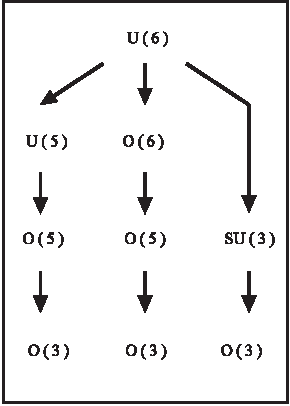
\includegraphics[scale=.65]{figure}
%
% If not, use
%\picplace{5cm}{2cm} % Give the correct figure height and width in cm
%
\caption{Please write your figure caption here}
\label{fig:A1}       % Give a unique label
\end{figure}

% For tables use
%
\begin{table}
\caption{Please write your table caption here}
\label{tab:A1}       % Give a unique label
%
% For LaTeX tables use
%
\begin{tabular}{p{2cm}p{2.4cm}p{2cm}p{4.9cm}}
\hline\noalign{\smallskip}
Classes & Subclass & Length & Action Mechanism  \\
\noalign{\smallskip}\hline\noalign{\smallskip}
Translation & mRNA$^a$  & 22 (19--25) & Translation repression, mRNA cleavage\\
Translation & mRNA cleavage & 21 & mRNA cleavage\\
Translation & mRNA  & 21--22 & mRNA cleavage\\
Translation & mRNA  & 24--26 & Histone and DNA Modification\\
\noalign{\smallskip}\hline\noalign{\smallskip}
\end{tabular}
$^a$ Table foot note (with superscript)
\end{table}
%


\backmatter%%%%%%%%%%%%%%%%%%%%%%%%%%%%%%%%%%%%%%%%%%%%%%%%%%%%%%%

% \Extrachap{Solutions}

\section*{Problems of Chapter~\ref{intro}}

\begin{sol}{prob1}
The solution\index{problems}\index{solutions} is revealed here.
\end{sol}


\begin{sol}{prob2}
\textbf{Problem Heading}\\
(a) The solution of first part is revealed here.\\
(b) The solution of second part is revealed here.
\end{sol}


% \printindex

%%%%%%%%%%%%%%%%%%%%%%%%%%%%%%%%%%%%%%%%%%%%%%%%%%%%%%%%%%%%%%%%%%%%%%
\biblstarthook{}

\begin{thebibliography}{99.}%
% and use \bibitem to create references.
%
% Use the following syntax and markup for your references if 
% the subject of your book is from the field 
% "Mathematics, Physics, Statistics, Computer Science"
%

\bibitem{g1957} Grothendieck, Alexandre. "Théorèmes de dualité pour les faisceaux algébriques cohérents." Séminaire Bourbaki 149 (1957): 25.
\bibitem{g1958} Grothendieck, Alexander. "The cohomology theory of abstract algebraic varieties." Proceedings of the International Congress of Mathematicians. 1958.
\bibitem{s1959} Serre, J-P. "Groupes algébriques et corps de classes." Hermann (1959).
\bibitem{report1956} Zariski, Oscar. "Scientific report on the second summer institute, several complex variables. Part III. Algebraic sheaf theory." Bulletin of the American Mathematical Society 62.2 (1956): 117-141.
\bibitem{z1952} Zariski, Oscar. "Complete linear systems on normal varieties and a generalization of a lemma of Enriques-Severi." Annals of Mathematics (1952): 552-592.
\end{thebibliography}

\end{document}





